% A skeleton file for producing Computer Engineering reports
% https://kgcoe-git.rit.edu/jgm6496/KGCOEReport_template

\documentclass[CMPE]{KGCOEReport}

% The following should be changed to represent your personal information
\newcommand{\classCode}{CMPE 663}  % 4 char code with number
\newcommand{\name}{Andrei Tumbar}
\newcommand{\LabSectionNum}{1}
\newcommand{\LabInstructor}{Wolfe}
\newcommand{\TAs}{Nitin Borhade}
\newcommand{\exerciseNumber}{5}
\newcommand{\exerciseDescription}{Signal Generator}

\usepackage{tikz}
\usepackage{circuitikz}
\usetikzlibrary{calc}
\usepackage{multirow}
\usepackage{titlesec}
\usepackage{float}
\usepackage{lmodern}
\usepackage{pgfplots}
\usepackage{siunitx}
\usepackage{subcaption}
\usepackage{graphicx}
\usepackage[usestackEOL]{stackengine}
\usepackage{scalerel}
\usepackage[T1]{fontenc}
\usepackage{amsmath}


\def\code#1{\texttt{#1}}

\begin{document}
    \maketitle
    \section*{Analysis/Design}

    This project looked at generating certain waveforms with varying parameters.
    The usage of the DMA in tandem with the DAC was crucial to the operation of
    this exercise. A system was designed in which the DAC could be utilized to
    its maximum operating speed when enough RAM was available.

	\begin{figure}[h!]
      \centering
      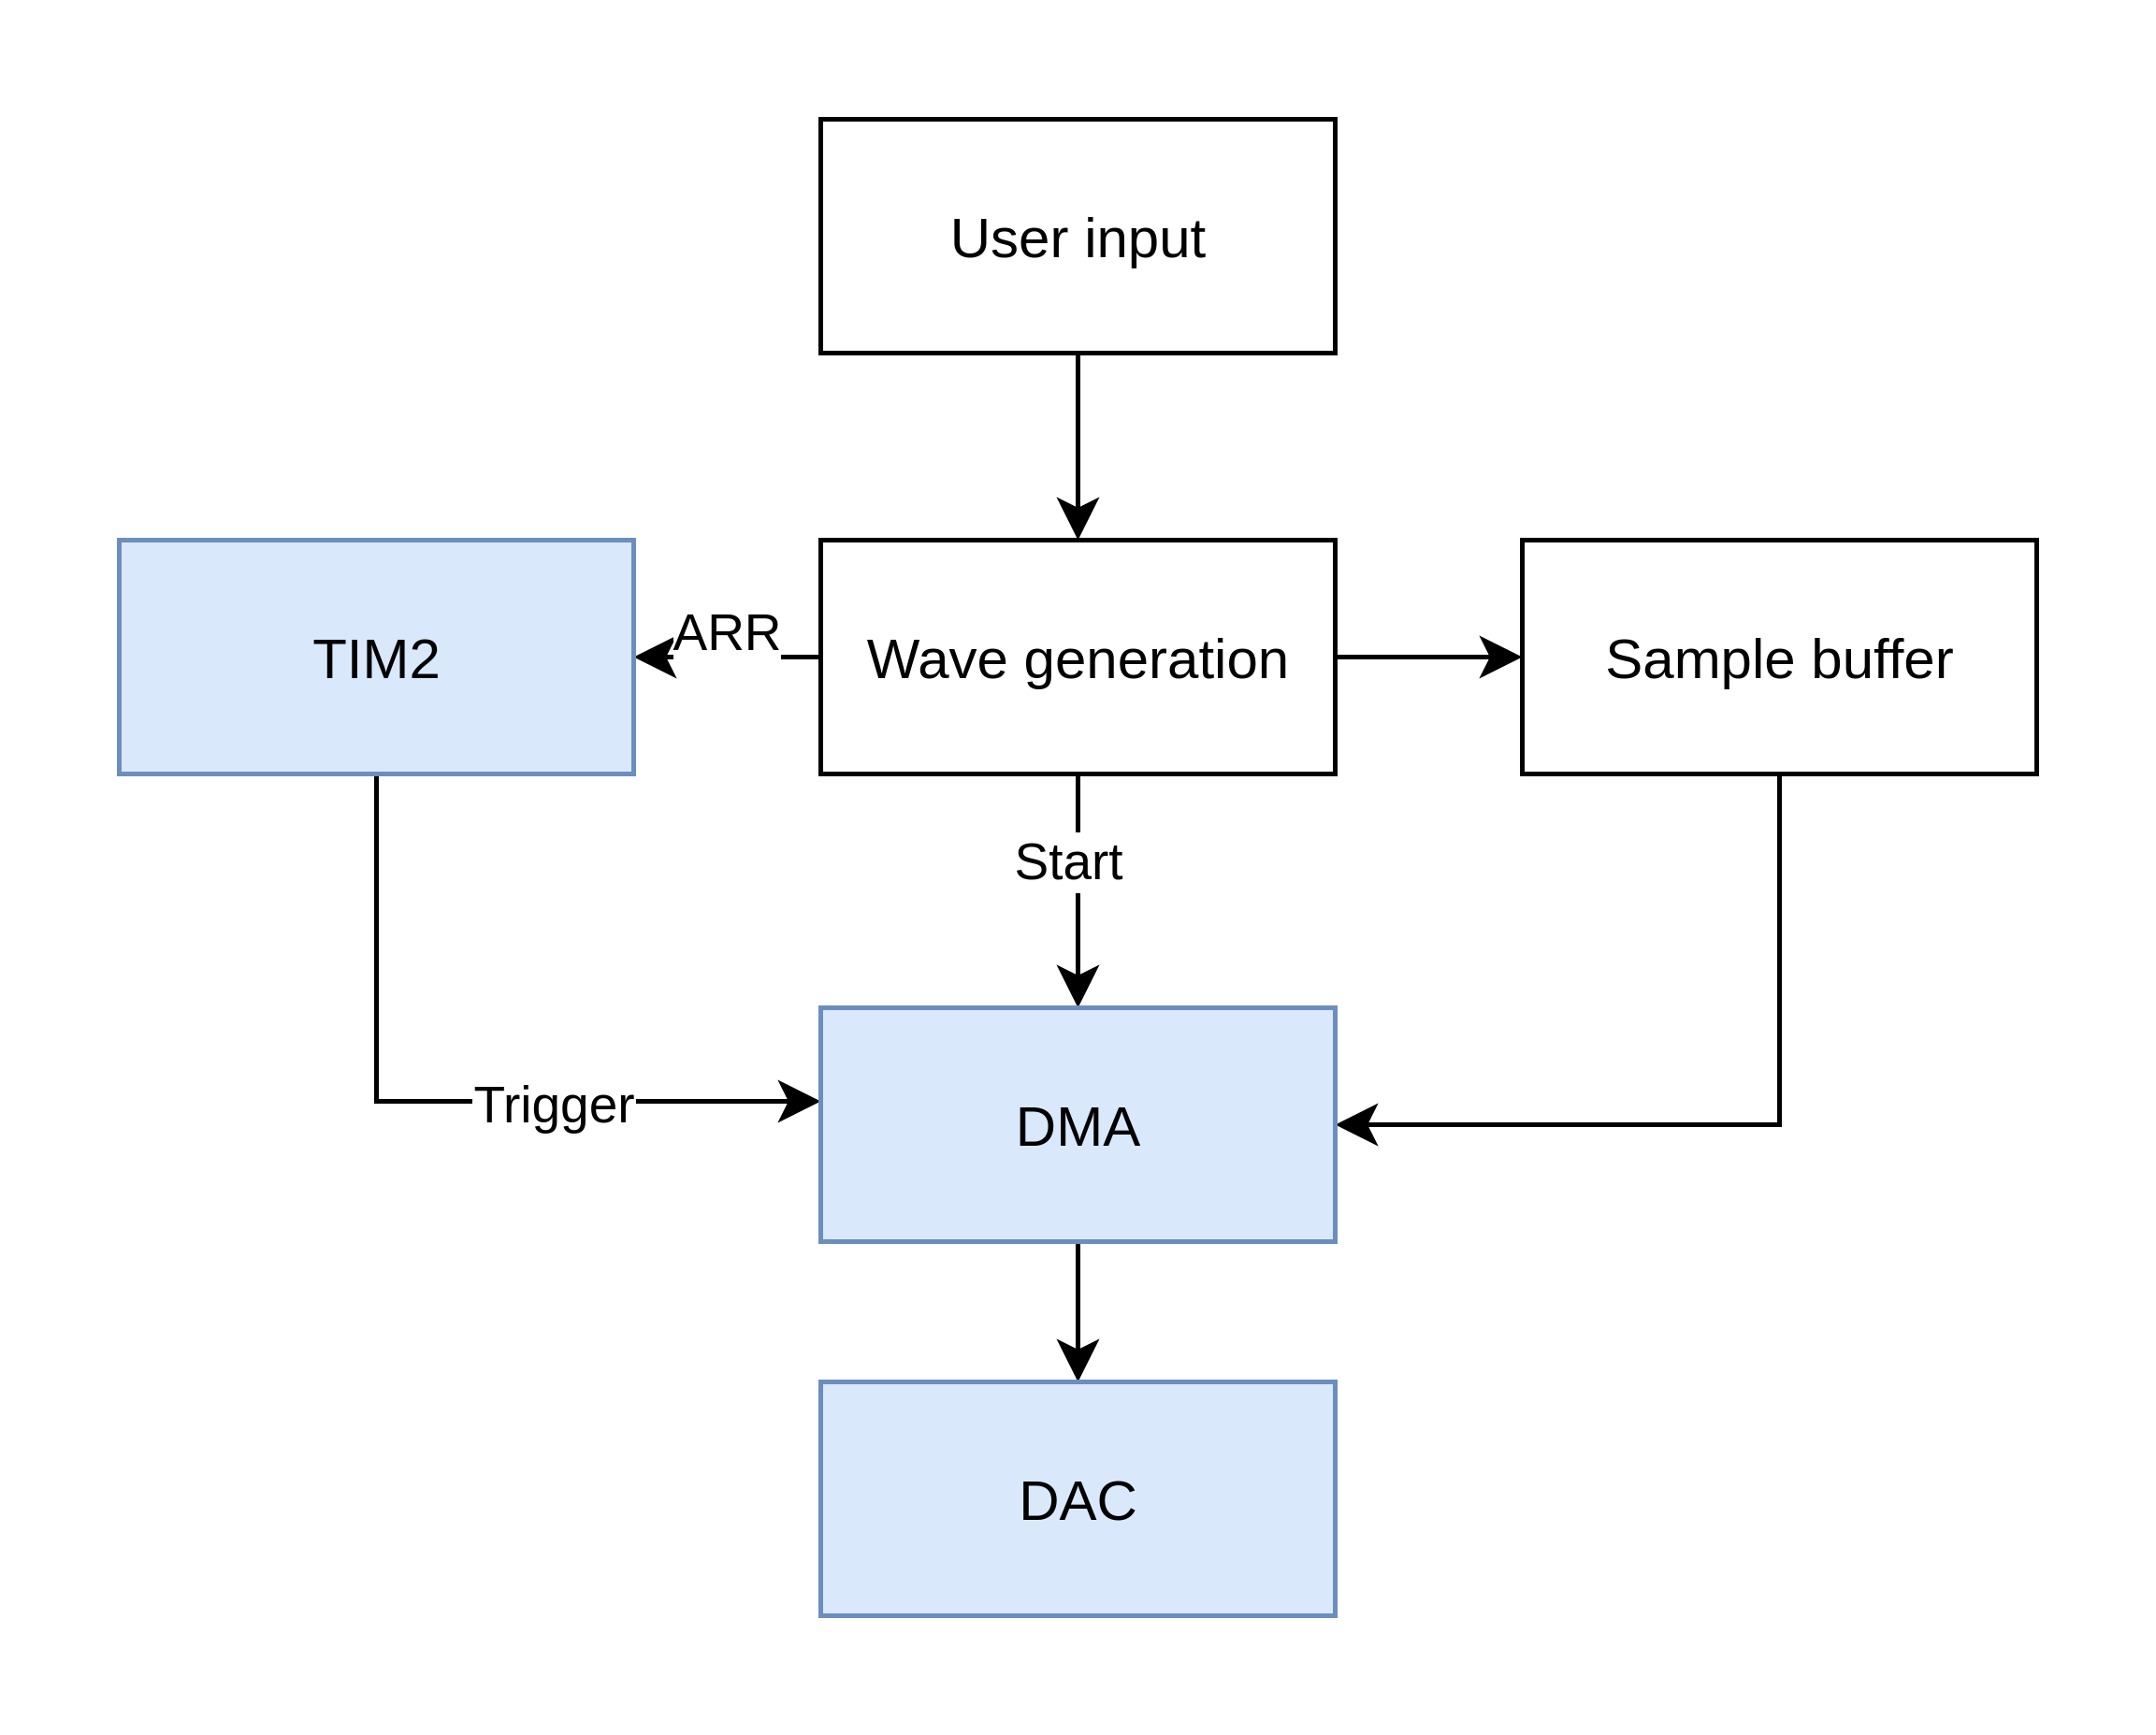
\includegraphics[width=12cm]{overview}
      \caption{Overview of system operation}
      \label{fig:overview}
    \end{figure}

	

	\subsection*{Hardware Operation}

	The signals that must be generated for this project need to reach a maximum
	of \SI{100}{\kilo\Hz}. Unlike the previous project, operating the DAC using
	a timer interrupt will not work properly at this frequency. Interrupting the
	CPU causes inherent delay that will far exceed the minimum response time at
	the maximum frequency. To circumvent this issue, the DMA may be used to write
	to the DAC directly. The DMA peripheral must be triggered by a hardware source
	to operate in the way we intend. \code{TIM2} was used again to trigger the DMA.
	Like the previous project, we can represent the frequency of a discrete periodic
	wave given the trigger frequency and number of buffer samples.

	\begin{equation}
	F_{sysclk} = F_{wave} \cdot N_{samples} \cdot (ARR + 1)(PSC + 1)
	\end{equation}

	For now we will assume that the DAC may operate at an arbitrarily high
	frequency and we will account for this later on. $F_{sysclk}$, $F_{wave}$,
	and $N_{samples}$ are known constants. $ARR$ and $PSC$ are variables. In the
	previous project we set, $PSC = ARR$. However this method will not allow the
	accuracy at higher frequencies. We are now setting $PSC=0$.

	\begin{align}
	ARR &= \frac{F_{sysclk}}{F_{wave} \cdot N_{samples}} - 1
	\end{align}

	We assumed previously that the DAC may operate at an arbitrarily high rate.
	This is not an accurate assumption as the DACs on the this STM32 board have
	a maximum sample rate of \SI{1}{\mega SPS}. Using the wave frequency, a known
	constant, we can calculate the maximum number of samples we can use inside
	a single period to reach the maximum sample rate of the DAC peripheral.

	\begin{align}
	N_{samples} = \frac{\SI{1}{\mega SPS}}{F_{wave}}
	\end{align}

	Because we don't have infinite memory and our sample buffer is statically
	allocated, we must cap the number of samples to the chosen length of the
	sample buffer. A sample buffer length of $2000$ was chosen because it
	creates a smooth curve at the minimum operating frequency and isn't too
	large.

	\subsection*{Wave Generation}

	To generate the waveforms for the triangular, square, and sinusoid, differing
	methods were used. The square wave was the simplest with half of the buffer
	being the maximum voltage and the other half being the minimum voltage. The
	triangle wave could be generated by calculating the slope between the min
	and max voltages over half of the usable buffer length. Then use this slope
	to interpolate a rising line in the first half and a mirrored falling line
	in the second half. Lastly, the sinusoid is generated by scalling the
	\code{sin()} function from the \code{math} library to the length of buffer.
	The move and scale this function to fit within the desired min/max range.

    \section*{Test Plan}

    To test operation, an oscilloscope was used to monitor the wave generation.
    The oscilloscope can measure periodic wave frequencies and was able to varify
    the correct operation of the system. To test, low frequencies were used first to
    verify that the chosen buffer length was long enough to create smooth curves.
    The highest frequencies were tested last to verify that the algorithm to determine
    the buffer length operated properly.

    \section*{Project Results}

	Results shown on the oscilloscope are expected. Low frequency waveforms have very
	smooth profiles while higher frequencies (higher than \SI{10}{\kilo\Hz}) start to
	show more jageddy edges. This is expected because the maximum sample rate of the
	DAC peripheral begins to have significant impact waveforms profile. At the highest
	frequency (\SI{100}{\kilo\Hz}), we can see that only about 10 samples are used which
	create step like function for the triangular and sinusoidal waveforms. The square
	wave does not suffer at all from the lower sample count as it only requires two
	samples to fully model the waveform.

    \section*{Lessons Learned}

	This project explored the operation of the DMA in conjuction with the DAC. When
	starting the project, following a DMA/DAC setup guide for STM32 did not work at
	all. There turned out to be a completely unrelated peripheral accessing the GPIO
	bus causing the DMA to not play nicely with the DAC. Starting the project from
	scratch and not initializing peripherals to their defaults allowed the DMA to work
	as intended. The second major obstacle was finding out that the DAC had a maximum
	sample rate. Deriving an algorithm to limit trigger frequency of the timer by limiting
	the number of samples used was vital in making this project as robust as possible.

\end{document}
